% This is LLNCS.DEM the demonstration file of
% the LaTeX macro package from Springer-Verlag
% for Lecture Notes in Computer Science,
% version 2.3 for LaTeX2e
%
\documentclass[11pt]{llncs}
%
\pagestyle{plain}
\usepackage{makeidx,graphicx,amsmath,verbatim}  % allows for indexgeneration
\usepackage[vlined, ruled]{algorithm2e}


%
\setlength{\topmargin}{-0.3in}
\setlength{\textheight}{8.75in}
\setlength{\oddsidemargin}{0.25in} 
\setlength{\evensidemargin}{0.25in} 
\setlength{\textwidth}{6.00in}

\begin{document}

%
%
\mainmatter              % start of the contributions
%
\title{Hapler Version 1.60}
%
%\titlerunning{Hapler Version 1.01}  % abbreviated title (for running head)
%                                     also used for the TOC unless
%                                     \toctitle is used
%
\author{Shawn T. O'Neil \and Scott J. Emrich}
%
\authorrunning{Shawn T. O'Neil et al.}   % abbreviated author list (for running head)
%
%%%% list of authors for the TOC (use if author list has to be modified)
\tocauthor{Shawn T. O'Neil, Scott J. Emrich}
%
\institute{University of Notre Dame, Notre Dame, IN 46556, USA\\
	\email{\{soneil,semrich\}@nd.edu} 
	}




\maketitle              % typeset the title of the contribution


\setcounter{tocdepth}{3}
\tableofcontents

\newpage

%\begin{abstract}

%\end{abstract}
%

\section{Overview} 
\label{overview}

Suppose you are given a alignment of sequencing reads (such as those that contribute to a consensus contig in an assembly, or a mapping of reads against 
a reference, see Section 
\ref{inputAndOptions}) that represent and unknown number of haplotypes. For example, perhaps you have pooled material for a number of (non-clonal) 
individuals and you sequenced from the ND5 gene of each and aligned them to a reference. Hapler is a tool that attempts to assemble these 
haplotypes individually. If there is enough information (high enough coverage, long enough reads, low enough error rates, high enough differentiating 
diversity in the dataset), there is a good chance this can be done. If not, Hapler takes care to only assembly shorter haplotype regions it is 
``sure'' of.

Once these haplotype regions are assembled, Hapler also reconstructs an overall consensus that attempts to minimize and identify points of
possible chimerism (points in the 
consensus where different SNPs must be supported by different haplotype regions).

For a quick introduction into the basic use of Hapler see Section \ref{exampleUsage}. For considerations on maximizing quality, see section 
\ref{maximizingQuality}.






\newpage
\section{Changelog}
\label{changelog}



	  \subsection*{1.6}
\begin{itemize}	  
\item Added a new SNP caller, which has been set as the default: binomial.
\end{itemize}


	  \subsection*{1.55}
\begin{itemize}	  
\item Fixed a bug in reading ground truth alignments.
\item Added internal book-keeping for allele counts to SNPs.
\item Fixed a bug in the SAM parser: sam files are 1-indexed, hapler is 0 indexed.
\item Added two new columns of output when using --ground-truth option (closest grount truth match, and number of differences from closest match).
\end{itemize}


	  \subsection*{1.54}
\begin{itemize}	  
\item Fixed a small bug in the 454 snp caller where overlapping homopolymer run errors might be called as SNPs.
\end{itemize}

	  \subsection*{1.53}
\begin{itemize}	  
\item Tweaked the output format and warnings format (again) for ease of description and parsing.
\item Implemented custom SNP loading from a text file (finally).
\item Removed the \texttt{--allow-gaps} option; by default gaps are split and mate-pair information is ignored; a warning is output when this happens.
\end{itemize}

	  \subsection*{1.52}
\begin{itemize}	  
\item Adjusted the output format to be more parseable, hopefully.
\item Added an optional \texttt{--human-readable} option to decrease output size for large datasets.
\item Fixed a bug where the program would crash when given an alignment with no SNPs.
\item Code cleanup and fixes.
\end{itemize}

	\subsection*{1.51}
\begin{itemize}
\item Fixed bug with parsing SAM format, if cigar string is ``*'', the read is skipped.
\end{itemize}

	\subsection*{1.5}
\begin{itemize}
\item Internal logic cleanup
\item Added \texttt{auto} option for \texttt{--random-repetitions}. 
\item Added \texttt{--max-repetitions} option.
\item Added minimum-chimerism consensus reconstruction, evaluation of given contig consensuses and majority vote.
\item Fixed an error in the 454 SNP caller where SNPs could be called even if the majority vote was a gap.
\end{itemize}

	\subsection*{1.01}
\begin{itemize}
\item Added ability to have \texttt{\~}'s in TIGR formatted sequences, so that \texttt{--allow-gaps} (split) can be used with them).
\end{itemize}

	\subsection*{1.0}
\begin{itemize}
\item Initial release.
\end{itemize}




\newpage

\section{Requirements and Installation}
\label{requirementsAndInstallation}

Hapler is written in Java (as a single .jar file), and has been tested with Java 1.6.0\_22 (on OSX 10.6.6). It is released under the LGPL. To install
and use Hapler, one simply needs to acquire the .jar file and run \texttt{java -jar Hapler.jar} on the command line.





\newpage

\section{Example Usage} 
\label{exampleUsage}

The default parameter settings are such that Hapler will assemble haplotype regions and reconstruct a minimum-chimerism consensus in a conservative 
fashion for low diversity, low-coverage data (e.g., an arthropod EST sequencing project). Hapler reads TIGR formatted assemblies on standard input by 
default and uses the built in ``simplestrict'' SNP caller (requiring 2x coverage of the minority allele for calling SNPs, see section \ref{inputAndOptions}).

Thus, good results from Hapler should be attainable by running something as simple as:

\begin{verbatim}
 cat pz_p450_CP6B6_pop.tigr | java -jar Hapler.jar
\end{verbatim}

Reading on standard input isn't required, of course:

\begin{verbatim}
 java -jar Hapler.jar --input pz_p450_CP6B6_pop.tigr
\end{verbatim}

Looking at the result of the above by piping into \verb=less -S=, we can see that Hapler returns a lot of information in column/row format, with 
informative comments and warnings (lines starting with \verb=#= for easy filtering) describing each column. See Section \ref{output} for more detail about what is 
returned. In this case, because the data was generated by 454, we may wish to use the built-in 454 SNP caller (though for best results SNPs should be
called with external software and imported with \verb=--snp-caller=).

\begin{verbatim}
 cat pz_p450_CP6B6_pop.tigr | java -jar Hapler.jar --snp-caller 454
\end{verbatim}


Because Hapler outputs on standard out, we can easily do things such as filter down to haplotype assemblies (lines starting with \texttt{@}) with high coverage, which our experiments show tend to be
correct:

\begin{verbatim}
 cat pz_p450_CP6B6_pop.tigr | java -jar Hapler.jar --snp-caller 454 
                            | grep -v '^@' 
                            | awk '{if($16 > 2) print $0}'
\end{verbatim}


Perhaps we are only interested in the minimum-chimerism consensus reconstructions produced (lines starting with \texttt{>} with '\texttt{Hapler}' in the third column), and we want to create a fasta file from them:

\begin{verbatim}
 cat pz_p450_CP6B6_pop.tigr | java -jar Hapler.jar --snp-caller 454   
                                          (run Hapler)
                            | grep '^>'
                                          (Filter to consensus reconstructions)
                            | awk '{if($3 == "Hapler") print $0}'     
                                          (Isolate Hapler Consensuses)
                            | awk '{print $1,$2,$3,$4,$5,$6,$7"\n"$8}' 
                                          (Print in fasta format)
                            > pz_hapler.fasta
\end{verbatim}


\newpage
Because Hapler can read on standard input, one can easily run Hapler on contigs in an Amos Bank. 
For example, if the file \texttt{eidlist.txt} contains a number of contig identifiers
associated with the Amos Bank \texttt{bank}, one can simply run:

\begin{verbatim}
bank2contig -E eidlist.txt bank | java -jar Hapler.jar --snp-caller 454
\end{verbatim}

Or, using command line sub-shells, two specified contigs:

\begin{verbatim}
bank2contig -E <(echo 7180000019110\\n7180000019111) bank 
                                       | java -jar Hapler.jar --snp-caller 454
\end{verbatim}



\newpage

\section{Input and Options}
\label{inputAndOptions}

Hapler reads multiple alignments in TIGR format (produced by the Amos tools \verb=bank2contig= utility) or SAM format. For examples of these two 
formats, see Appendix \ref{exampleTigrInputFormat} and \ref{exampleSamInputFormat}. If you find bugs in inputting these formats, please let us know. 
Note that Hapler does \emph{not} do the assembly or alignment step for you: you need to produce a TIGR or SAM formatted multiple alignment file 
(either via de-novo assembly or mapping to a reference).

Hapler assumes that \verb=~= characters in either SAM or TIGR sequences are gaps. Otherwise, Hapler is alphabet agnostic: any other non-whitespace
non\verb=~= character can be used in the multiple alignments (for example, one could ``haplotype'' protein sequences). 

Although TIGR format does not describe mate-pair information (that we are aware of), SAM format may. Because gaps (e.g. mate-pair information) are 
not compatible with the minimum coloring process (in polynomial time), Hapler will split sequences containing \texttt{\~} characters into multiple
sequences and will ignore all mate pair information. If this happens, a warning is printed to the output. 


Hapler takes the following options:

\subsection{\texttt{--input <filename or \emph{-}>}}

The name of the alignment file (SAM or TIGR) to use. If `-' is used (which is the default), Hapler reads on standard input.

\subsection{\texttt{--alignment-type <\emph{tigr} or sam>}}

Values can be either \verb=tigr= or \verb=sam=, depending on input type. The default is \verb=tigr=, note that input type is \emph{not}
autodetected.

%\subsection{\texttt{--allow-gaps <\emph{false} or split>}}

%Values can be either \verb=false= (the default), or \verb=split=. Using a value of \verb=false=, Hapler will exit with an error
%if any sequence contains a gap character \verb=~= or the SAM format describes mate-pair information. Using \verb=split= causes gapped data
%to be split into component contiguous sequences (and mate-pair information to be ignored). 

\subsection{\texttt{--help}}

Shows a brief description of Hapler and options.


\subsection{\texttt{--maximize-one-read-haps <\emph{true} or false>}}

As mentioned in Section \ref{howItWorks}, Hapler samples from minimum colorings of each connected component of the conflict graph.
By default, Hapler searches for minimum colorings which also maximize the number of reads that get colors to themselves: we argue that
since some reads are likely to contain sequencing errors, we have a better chance of isolating them by searching for haplotypes that can 
consist of a single read within the parsimony framework of minimum coloring.

This can be turned off by setting this value to false.

\subsection{\texttt{--random-repetitions \emph{auto} or <integer>}}

As mentioned in Section \ref{howItWorks}, Hapler samples from minimum colorings of each connected component of the conflict graph.
By repeating these samples and only putting reads together into the same haplotype if they \emph{always} appear together in all
sampled colorings, we can be more sure of the quality of the inference. By increasing the number of samples, we can increase the robustness,
usually at the cost of haplotype length.

By default (\texttt{auto}), Hapler runs 20 repetitions, and continues running repetitions until either 1) the last 50\% of repetitions has not resulted
in more haplotype reconstructions, or 2) the maximum number of repetitions is reached (default 100).

\subsection{\texttt{--max-repetitions <integer>}}

The maximum number of repetitions to run, even if \texttt{random-repetitions} is \texttt{auto}, default 100.


\subsection{\texttt{--snp-caller <simple, simplestrict, 454, or \emph{binomial}>}}

For best results, one should use the \emph{--snp-list} option, which overrides this one. Nevertheless, Hapler provides several simple SNP 
calling methods, outlined below:

\begin{itemize}
	\item \texttt{simple}: Any variant locus regardless of allele frequency is treated as a SNP locus.
	\item \texttt{simplestrict}: Any variant locus where a minority allele is present at least twice or is covered by less than 10 reads is treated as a SNP.
	\item \texttt{454}: A variant locus is a SNP if 1) the majority allele is not a `$-$'
	and 2) either a) the number of non-`$-$' alleles is at least two, or
	b) there is any non-`$-$' allele that is not part of a homopolymer run
	of length $\geq 3$.
	\item \texttt{binomial} (default): Given an estimated error rate $e$ (default 0.005) and sequence alphabet $A$, at a non-polymorphic locus the
   expected occurrence rate of the second most frequent character (under an equal substitution model) will be $e/(|A|-1)$. Thus, this method
   uses a Bonferroni corrected Binomial test to call SNPs: for each locus, we call a SNP if the actual second most frequent character count is
   greater than $F^{-1}\left(1-\alpha/L; d, e/(|A|-1) \right)$, where $F^{-1}$ is the inverse cumulative Binomial distribution function, 
   $\alpha$ is the p-value cutoff (default 0.05), $L$ is the length of the alignment, and $d$ is the read depth at the locus. The alpha value 
   and expected error rate can be controlled with the options \texttt{--binomial-alpha} and \texttt{--binomial-error-rate}.
\end{itemize}


Because the results are fairly dependent on SNP calling and/or error correction accuracy (both in terms of false positives and false negatives), it would
be wise to see section \ref{maximizingQuality}.


\subsection{\texttt{--binomial-alpha <float>}}

Controls the multiply-corrected p-value cutoff for calling SNPs using the binomial SNP caller. See input for \texttt{--snp-caller} for more information.

\subsection{\texttt{--binomial-error-rate <float>}}

Controls the estimated error rate for calling SNPs using the binomial SNP caller. See input for \texttt{--snp-caller} for more information.

\subsection{\texttt{--snp-list <filename>}}

Rather than use the simple built in SNP callers that Hapler provides, the user can provide a list of (0-indexed) loci that describes positions to
use as SNP loci for each multiple alignment. 

This is useful when using external SNP callers, such as QualitySNP or PyroBayes.

For an example of the format taken, see Appendix \ref{exampleSnpInputFormat}.

\subsection{\texttt{--ground-truth <filename>}}

If the actual full length haplotypes the reads are sourced from are known (as in simulation or testing), they can be provided to Hapler. In this
case, all reconstructed and evaluated consensus sequences (Hapler generated, Majority Vote, and Contigs given for evaluation), as well as all
assembled haplotype regions, will be evaluated for chimerism and agreement with the ground truth haplotypes. This information will result
in extra columns being added to the output.

This option requires a fasta file containing the haplotypes, all of which need to be the same length as the alignment. Note that these haplotypes
are used for comparison in all alignments. Thus, this option is only really useful when the input describes a single alignment.

\subsection{\texttt{--evaluate-contigs <filename>}}

For each alignment, Hapler can evaluate a given consensus contig (which must be the same length as the alignment) for chimerism. Hapler
estimates the minimum number of crossover points needed reconstruct the contig using Hapler assembled haplotype regions (where a crossover
point is a pair of SNPs that cannot be supported by a single haplotype region). If the \texttt{--ground-truth} option is used, the contig is 
also evaluated against the ground truth haplotypes. 

The input for this option should be a fasta file with sequences corresponding to alignments having the same ID. Contigs must the same length
as the alignments they represent.

\subsection{\texttt{--compute-reconstructions <\emph{true} or false>}}

By default, Hapler reconstructs a minimum-chimerism consensus sequence from the haplotype regions and evaluates the chimerism of it against the
haplotype regions as well as against ground truth haplotypes (if given). It also reconstructs the majority vote consensus and evaluates the chimerism
against Hapler haplotype regions as well as against ground truth. For long alignments with many SNPs, this process can be computationally expensive 
($O(\#SNPs \times \#Haplotypes^2)$): this option allows the user to turn it off.

\subsection{\texttt{--human-readable <\emph{true} or false>}}

By default, Hapler outputs haplotype region assemblies in human readable format: aligned against each other and padded with \~ characters, including a line
indicating where SNPs occur. For long alignments with many short haplotype regions, this results in the output containing mostly padding, which can take
a long time to output and takes up a lot of space. This option removes the padding and the SNP identification line.


\subsection{\texttt{--show-alignments}}

Mostly for debugging, this option reports the sections of the multiple alignment contributing to each haplotype reconstruction. Currently
not very user-friendly.


\subsection{\texttt{--version}}

Output version information and exit.

\newpage


\section{Output}
\label{output}

At the start of every run, hapler outputs comment lines (prefixed with \texttt{\#\#}) that describe the further output of Hapler in short form. Hapler
also outputs running information to standard out.

By default, Hapler outputs results in rows and human readable columns (try using \texttt{less -S} to view the output), with each row 
corresponding to either warnings or messages, assembled haplotype regions, or full-alignment-length consensus sequences. 

Specifically, for each alignment, hapler outputs 

\begin{enumerate}
\item Warnings, if appropriate, prefixed with \texttt{\#!}. (These usually refer concerns about SNP calling, for example, if an alignment appears to have no SNPs.)
\item A number of lines corresponding to consensus sequences and their chimerism evaluation, prefixed with \texttt{>} (Hapler generated, Majority vote, and provided contigs if the \texttt{--evaluate-contigs} option was used).
\item A line describing the positions of called SNPs, prefixed with \verb=#*=
\item A line representing the ``universal'' haplotype region, containing reads that are consistent with all haplotypes, prefixed with \texttt{@@}.
\item A number of lines each corresponding to an assembled haplotype region, prefixed with \texttt{@}. 
\end{enumerate}

\begin{figure}[!h]
\centering
   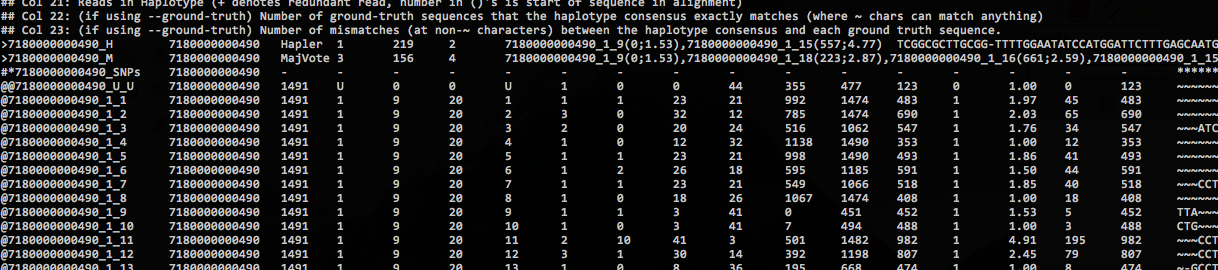
\includegraphics[width=\textwidth]{graphics/hapler_output}
   \caption{A bit of output produced by Hapler.}
   \label{haplerOutput}
\end{figure}

\newpage
\subsection{Consensus Sequence Output Lines}

\subsubsection{Consensus (\texttt{>} prefixed) Column 1 - Unique Consensus Identifier}

This column gives a unique identifier for each reconstructed haplotype region, which is merely a concatenation of the alignment name and
a code for the consensus type (H for Hapler generated, M for majority vote, C for evaluated contig).


\subsubsection{Consensus (\texttt{>} prefixed) Column 2 - Alignment Name}

The name of the alignment this consensus is associated with.

\subsubsection{Consensus (\texttt{>} prefixed) Column 3 - Consensus Type}

``Hapler'' for Hapler generated consensus, ``MajVote'' for the majority vote, ``Contig'' for evaluated contigs given by \texttt{--evaluate-contigs}.

\subsubsection{Consensus (\texttt{>} prefixed) Column 4 - Minimum Hapler Crossovers}

This column gives the minimum number of crossovers necessary to reconstruct the consensus sequence from Hapler assembled haplotype regions. Here, a 
crossover is defined as an adjacent pair of SNPs that are not both supported by some haplotype region. Note that Hapler optimizes its consensus 
sequence according to this (and the following) criterion, so it will necessarily have the lowest value. Also note that any allele in a consensus at a 
SNP position that is not represented in any haplotype region (i.e., is novel, and is likely an error), is treated as being supported by a ``unique'' 
haplotype specific to that locus, and hence incurs two crossovers: one into and one out of the unique haplotype (unless it is at the first of last 
SNP).

This column thus represents Hapler's estimate of the ``chimerism'' of the consensus sequence. Note that because Hapler is conservative in 
assembling haplotype regions, this number almost always overestimates the true chimerism (unless Hapler is made less conservative by using a very
small number for the \texttt{--random-repetitions} options).

\subsubsection{Consensus (\texttt{>} prefixed) Column 5 - Maximized SNP Allele Support}

After finding the minimum number of crossovers necessary to reconstruct a consensus, Hapler adjusts these crossovers to maximize the total number of
bases (in redundant and non-redundant reads) supporting the consensus in haplotype regions. More formally, if haplotype $s(i)$ is chosen to support
a SNP locus $i$, and haplotype $s(i)$ has coverage of $c(s(i))$ at this locus, this column maximizes $\sum_{i \in SNPs}c(s(i))$.

\subsubsection{Consensus (\texttt{>} prefixed) Column 6 - Minimized Unique Haplotype Regions Used}

After minimizing chimerism and maximizing support of a consensus, Hapler seeks to minimize the number of unique haplotype regions used
to reconstruct a consensus. This tie-breaking criterion will seldom discriminate between two reconstructions in practice.

\subsubsection{Consensus (\texttt{>} prefixed) Column 7 - Hapler Haplotype Regions Used}

Hapler optimizes several criteria (above) to determine which haplotype regions should be used at SNP positions to reconstruct a consensus sequence 
(non-snp positions are assumed to be supported by the majority vote or universal haplotype). This column lists which haplotype regions are chosen, 
where they start in the alignment (0-indexed), and what their average coverage is.

The start positions in this column are useful for determining where possible crossover points may occur. One may wish to mask these positions when designing
PCR primers or microarray probes, for example. 

\subsubsection{Consensus (\texttt{>} prefixed) Column 8 - Consensus Sequence}

The consensus sequence, as reconstructed from the haplotype regions used (for the Hapler generated consensus), the majority vote (for the MajVote 
consensus), or as given in the \texttt{--evaluate-contigs} option.

\subsubsection{Consensus (\texttt{>} prefixed) Column 9 - Ground Truth Minimized Crossover Number}

This column is only output if the \texttt{--ground-truth} option is used.

Hapler can evaluate its own consensus (or any consensus) not only against its own assembled haplotype regions, but also against a given set of ground 
truth sequences. As above, this column represents the minimum number of crossovers necessary to reconstruct the consensus, but out of the ground truth
sequences. 

This column thus represents the ``true'' level of chimerism. 

\subsubsection{Consensus (\texttt{>} prefixed) Column 10 - Ground Truth Minimized Unique Haplotypes Used}

This column is only output if the \texttt{--ground-truth} option is used.

First, note that each ground truth haplotype, being a single sequence, has a ``coverage'' of 1. Thus, the summed support is equal for all 
reconstructions and this secondary optimization is not done.

Instead, Hapler skips directly to minimizing the number of unique ground truth haplotypes needed to reconstruct the consensus. 

\subsubsection{Consensus (\texttt{>} prefixed) Column 11 - Ground Truth Haplotypes Used}

This column is only output if the \texttt{--ground-truth} option is used.

After optimizing the above criteria to determine which ground truth haplotypes are needed to reconstruct the consensus, Hapler outputs which ones
are used as well as their start positions for reference. These are the of ``true'' (minimum number of) chimerism points.

\newpage
\subsection{Haplotype Region Output Lines}

\subsubsection{Haplotype (\texttt{@} prefixed) Column 1 - Unique Haplotype Identifier}

This column gives a unique identifier for each assembled haplotype region, which is merely a concatenation of the next three columns.

\subsubsection{Haplotype (\texttt{@} prefixed) Column 2 - Alignment Name}

Each assembled haplotype region is associated with its input multiple alignment name (from the TIGR or SAM file) through this column.

\subsubsection{Haplotype (\texttt{@} prefixed) Column 3 - Alignment Length}

The length of the input alignment (also the length of the output consensus sequences).


\subsubsection{Haplotype (\texttt{@} prefixed) Column 4 - Haplotype Block Number}

Non-variant regions separate connected components in the conflict graph (see Section \ref{howItWorks}). When there are such non-variant regions 
(multiple connected components), we have no information to attach haplotypes from one variant region to another. Thus, each haplotype region is 
associated with a connected component of the conflict graph, or ``Haplotype Block,'' it belongs to through this column. These are numbered, for each 
multiple alignment, beginning at 1.

This value is `U' for the ``non-variant'' Haplotype, which is associated with a unique ``universal'' block. (But note that this block \emph{can} be 
associated with all other blocks, as we know that non-variant sequences can be phased with all haplotypes).

\subsubsection{Haplotype (\texttt{@} prefixed) Column 5 - Minimum Number of Haplotypes Supported By Block}

Parsimony suggests that we should minimally color the conflict graph (see Section \ref{howItWorks}), equivalent to reconstructing a 
minimum number of haplotype regions supported by the data. However, because we repeat and sample the coloring process, we usually
end up with a larger number of haplotype reconstructions. This number, which is the same for all haplotypes in a single block (it's really
associated with the haplotype block, rather than each haplotype region), gives the minimum number that would be constructed by pure parsimony (
i.e., this is the number of haplotype regions that would be created for this block if \texttt{--random-repetitions} was set to 1).

\subsubsection{Haplotype (\texttt{@} prefixed) Column 6 - Number of Repetitions Completed}

By default, for each haplotype block, Hapler repeats the coloring process in pseudo-random until no new haplotype regions are reconstructed
(see input section \texttt{--random-repetitions}). This column outputs the actual number of repetitions used for each haplotype block.

\subsubsection{Haplotype (\texttt{@} prefixed) Column 7 - Haplotype Region Number}

Within each haplotype block, each haplotype region is given a number, counting upward from 1. The ``non-variant'' haplotype is given the special
designator `U'.

\subsubsection{Haplotype (\texttt{@} prefixed) Column 8 - Number of Non-Redundant Sequences}

In order to minimally color the conflict graph, Hapler must ``mask'' redundant reads (those whose covered SNP loci are a subset of some other 
non-conflicting read). This masking is done by the reads themselves: if read A makes read B redundant, and read B makes read C redundant,
then A must also make C redundant: so A ``masks'' B and C and these are removed from the haplotyping process.

This column then gives the number of non-redundant (non-masked) reads associated with each haplotype reconstruction. (Note that for the universal
haplotype, all sequences are non-redundant.)

\subsubsection{Haplotype (\texttt{@} prefixed) Column 9 - Number of Redundant Sequences}

As a compliment to Column 6, we also give the number of redundant reads associated with reads contributing to each haplotype reconstruction.

\subsubsection{Haplotype (\texttt{@} prefixed) Column 10 - Number of Defined SNPs Covered}

A read is said to \emph{cover} a SNP locus if it has a known allele (non-`~' character) there. The number of SNPs defined by a haplotype region
is the union of those covered by all reads within it.

%\subsubsection{Column 9 - Number of Covered, Inconsistent SNPs}

%Currently, this value will always be 0. Future versions of Hapler may allow for the consideration of gapped reads (e.g. mate pair information), but 
%in this case some reconstructed haplotypes may contain conflicting alleles at SNP loci (since this breaks the minimum coloring foundations). This 
%column will count these inconsistencies.


\subsubsection{Haplotype (\texttt{@} prefixed) Column 11 - Number of Defined SNPs Not Covered}

The total number of defined SNPs for the alignment minus the number of defined SNPs covered. 


\subsubsection{Haplotype (\texttt{@} prefixed) Column 12 - Start Position of Haplotype Region}

This is the 0-indexed position of the first non-`~' character in the haplotype region assembly (i.e., the first position of the first read in the 
haplotype). If there are no reads in the haplotype region (this can only happen with the universal `U' haplotype region), this will be -1.

\subsubsection{Haplotype (\texttt{@} prefixed) Column 13 - End Position of Haplotype Region}

This is the 0-indexed position of the last non-`~' character in the haplotype region assembly (i.e., the last position of the last read in the haplotype).
If there are no reads in the haplotype (this can only happen with the universal `U' haplotype), this will be -1.

\subsubsection{Haplotype (\texttt{@} prefixed) Column 14 - Length of Haplotype Region}

End Position - Start Position + 1, unless no sequences are in the haplotype region (this can only happen with the universal `U' haplotype)), in which case 0.

\subsubsection{Haplotype (\texttt{@} prefixed) Column 15 - Number of Pieces Haplotype Is In}

Because of the minimum coloring formulation, it is possible for a haplotype to consist, for example, of only two reads that are far apart in the 
alignment and don't actually overlap. If these two always share a coloring, we can be confident of their association, even though there is no 
``positive'' information (shared SNP alleles) linking them (see Section \ref{howItWorks}).

Pieces represent association not only via coloring but also via positive shared SNP allele information: pieces are defined as connected components in 
an overlap-at-SNP loci graph within haplotype regions. Thus, for any two reads which are part of the same piece, there is a path over overlapping and 
agreeing SNP allele reads between them.

Multiple pieces indicate a lack of such positive information linking reads together within a reconstructed haplotype, even though the
repeated coloring may suggest they belong to the same haplotype.  Usually, however, the repetition
of colorings forces haplotypes down to a single piece.

\subsubsection{Haplotype (\texttt{@} prefixed) Column 16 - Average Sequence Coverage of Haplotype}

The is similar to the ``average gapped coverage'' used in assembly. We take the total number of bases represented in reads belonging to the haplotype
(\emph{including} redundant/masked reads), and divide it by the length of the haplotype (see above). Note that if a haplotype doesn't cover some
internal section (i.e., has internal `~' characters, which can only happen if it is in multiple pieces), then this value can be below 1.0.

\subsubsection{Haplotype (\texttt{@} prefixed) Column 17 - Base Coverage at SNP Positions}

Summing over SNP loci covered, we sum the number of reads belonging to the haplotype region that cover the locus. 

\subsubsection{Haplotype (\texttt{@} prefixed) Column 18 - Alignment Coverage}

The number of non-`~' characters in the haplotype region assembly. Note that this can be different than the haplotype region length (above) if
there are `~' characters in the middle of the haplotype region (which is rare).




\subsubsection{Haplotype (\texttt{@} prefixed) Column 19 - Haplotype Region Assembly at SNP Positions}

This column shows the assembled haplotype regions, with all non-SNP loci removed. It provides a good summary of the haplotype regions assembled and their
length/coverage at the important (variant) loci. These are shown aligned for all variant loci: where a haplotype doesn't determine an allele
a `~' character is used.

%Consensus bases for each SNP locus are called as the majority vote of reads within each haplotype (which will always agree unless there are Inconsistent
%SNPs, see above).

\subsubsection{Haplotype (\texttt{@} prefixed) Column 20 - Full Haplotype Region Assembly}

The column shows the assembled haplotype regions, including non-variant loci, all aligned against each other, padded with `~' characters (unless 
\texttt{--human-readable} is set to false). Where a haplotype isn't determined, `~' characters are used.

Consensus bases for each SNP locus are called as the majority vote of reads within each haplotype (which in fact always agree, so this 
majority vote is unanimous). Consensus bases for all other loci are called as the majority vote of all reads in the multiple alignment: this helps 
filter out sequencing errors which have not been called as SNP loci, since per-haplotype coverage is often low.

\subsubsection{Haplotype (\texttt{@} prefixed) Column 21 - Reads In Haplotype}

For each reconstructed haplotype, Hapler also reports the reads contributing to it. Read IDs that are prefixed with a `+' are redundant
and are masked by the preceding non-`+' read. For each read, the start position in the multiple alignment (0-indexed) is also given in 
parentheses. 

\subsubsection{Haplotype (\texttt{@} prefixed) Column 22 - Ground Truth Sequences Exactly Matched}

This column is only displayed when using the \texttt{--ground-truth} option.

If a set of ground truth haplotypes is given, then for each reconstructed haplotype region, hapler will count the number of ground truth haplotypes
for which it is a \emph{perfect} match, at all loci. Here, `~' characters in the haplotype region may match any character.

\subsubsection{Haplotype (\texttt{@} prefixed) Column 23 - Ground Truth Sequence Mismatch Counts}

This column is only displayed when using the \texttt{--ground-truth} option.

For each ground truth haplotype, Hapler indicates the number of mismatching bases that keep an assembled haplotype region from being a perfect
match. Thus, 0s indicate which ground truth haplotypes are perfect matches to the assembled haplotype region. This is evaluated over all 
loci, not just SNP loci.


\subsubsection{Haplotype (\texttt{@} prefixed) Column 24 - Minimum Ground Truth Sequence Mismatch Count}
\ \\
This column is only displayed when using the \texttt{--ground-truth} option.

Minimum mismatch count from column 23.

\subsubsection{Haplotype (\texttt{@} prefixed) Column 24 - Minimum Mismatch Ground Truth Sequence}
\ \\
This column is only displayed when using the \texttt{--ground-truth} option.

Ground truth haplotype achieving the minimum mismatch count from column 23.

\newpage
\section{Maximizing Quality}
\label{maximizingQuality}

In general, for haplotyping applications, poor data can result in 1) possible sequencing error being included in haplotype
assemblies, and 2) chimeric haplotype reconstructions. 
Hapler uses a repeated, weighted bipartite matching method to try and maximize the robustness of the returned haplotype regions (see Section 
\ref{howItWorks} and \cite{ONEIL2011}): although sequencing errors can still get through (these are often represented as single read 
haplotypes, and sometimes as longer haplotypes with low coverage) and chimeras can still exist, this usually results in shorter haplotypes being returned,
representing uncertainty in the data.

Thus, for best results, one should still consider the quality of data fed to Hapler.

\subsection{Read Length and Coverage}

If no read spans a non-variant region, Hapler will not attempt to build haplotypes across that region. Thus, it is necessary to 1) use long enough
read lengths that non-variant regions can be spanned by reads, and 2) have high enough coverage that this does actually happen. An estimation of 
read length and coverage necessary to do this can be found in \cite{ERIKSSON2008}. Ideally, one would want high enough coverage that all regions
of all haplotypes are covered to some degree. One of the benefits of Hapler is that if such data isn't available, it will work with what you do have
and not return answers that aren't well-supported.

\subsection{SNP Calling and Error Correction}

Our experiments with Hapler indicate that sequence quality and locating true SNPs is of quite high concern if one wants accurate haplotype 
reconstructions. Hapler determines errors from non-errors through the calling of SNP-loci: variations at SNP-called loci define the conflict 
information, while other variations (which are presumably errors) are ignored, though left in the original data.

Notably, both false-positive and false-negative SNP calls can adversely affect haplotyping performance. A false-negative SNP (a true SNP that is 
mistaken for a sequencing error) means that some genetic variation will be ignored. This can result in a haplotype missing from the output, or a 
possible chimera because that diversity may have allowed for differentiation that is consequently ignored.

False-positive SNPs (calling errors as SNPs) are troublesome as well---these can be viewed as erroneous, rare haplotypes supported by only a single 
read. This is variation that Hapler will attempt to isolate through the ``maximizing single-read haplotypes'' mechanism. Even so, it is possible for 
these erroneous reads to ``stick to'' other, correct reads that they share correct alleles with, resulting in longer (though usually low average 
coverage) haplotypes. Although a coverage-cutoff often identifies these (see \cite{ONEIL2011}), this is a waste of the correct reads that are 
stuck to the erroneous reads, reducing haplotype information amongst correct reads.

Finally, we note that calling SNPs is general much harder when coverage is low, as near the ends of assembled contigs. Thus, one may want to 
``trim'' alignments so that coverage is high throughout. Further, even if errors are not called as SNPs, if they sit in regions with locally low 
coverage (e.g., if there is a sequencing error in a locus only covered by two reads), Hapler may use the errors as the base call of the overall 
alignment, causing the error to be present in all haplotypes spanning that region.

\subsection{Sampling Number}

As described in Section \ref{howItWorks}, Hapler samples in a pseudo-random fashion from minimal coloring solutions, keeping only common
haplotype information: an increase in repetitions with the \texttt{--random-repetitions} parameter results in higher confidence of the
reconstructions. As shown in \cite{ONEIL2011}, for a single coloring many long but chimeric haplotypes are created. Increasing the
parameter to 5 rapidly decreased the number of such chimeras (at a cost of haplotype reconstruction length), and increasing to 10 further
improved the results but at a slower rate, becoming nearly asymptotic. 

By default, Hapler runs a minimum of 20 coloring repetitions, and continues running repetitions until the last 50\% of them have not
increased the number of haplotype regions reconstructed. However, in any case, Hapler will stop when \texttt{--max-repetitions} have 
been run (default 100).



 
\newpage

\section{How it works}
\label{howItWorks}

The following is a quick, intuitive overview. More details can be found in \cite{ONEIL2011}. We are grateful for the work done by Eriksson et al. 
(\cite{ERIKSSON2008}): Hapler expands on the initial graph-theoretical formulation proposed there for increased robustness on low-coverage, low-diversity
data.

Haplotyping is done primarily by creating a graph with each read corresponding to a node such that two nodes are connected by an edge if they conflict. If 
we minimally color this graph, each color consists of nodes that don't conflict and may represent data sourced from the same haplotype. Note that by this 
formulation reads which don't overlap can be given the same color, thus haplotype reconstructions can return ``gaps'' in the middle. For example the
``red'' reads in Figure \ref{exampleConflictGraph} leave an undefined section between the first and second read. This is infrequent in normal usage: 
\emph{usually} this indicates uncertainty caused by lack of coverage or genetic diversity which Hapler is designed to avoid (see below).

%% Figure of multiple coloring
\begin{figure}[!h]
\centering
   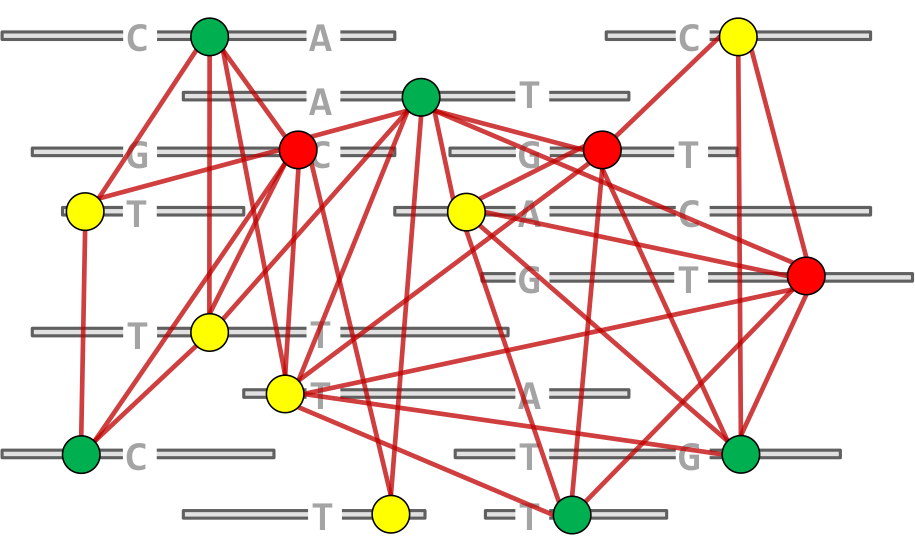
\includegraphics[width=0.4\textwidth]{graphics/mincolor}
   \caption{Given an alignment of reads (here showing only positions defined as SNPs), we want to create a conflict graph and minimally color it.}
   \label{exampleConflictGraph}
\end{figure}



Minimum coloring is generally NP-hard. However, if ``gaps'' (unknown sequence) are not allowed in the reads (where a gap in a read precludes 
conflicts at the unknown alleles), then this problem is polynomial time. Note that mate-pairs could be considered as single a single sequence with a 
large gap in the middle: ideally, we'd like to use a single graph node to represent both ends of the mated read. Unfortunately, to ensure polynomial 
time and correct answers, we have to use two nodes, thus each end may end up in different haplotype assemblies.

\begin{figure}[!h]
\centering
   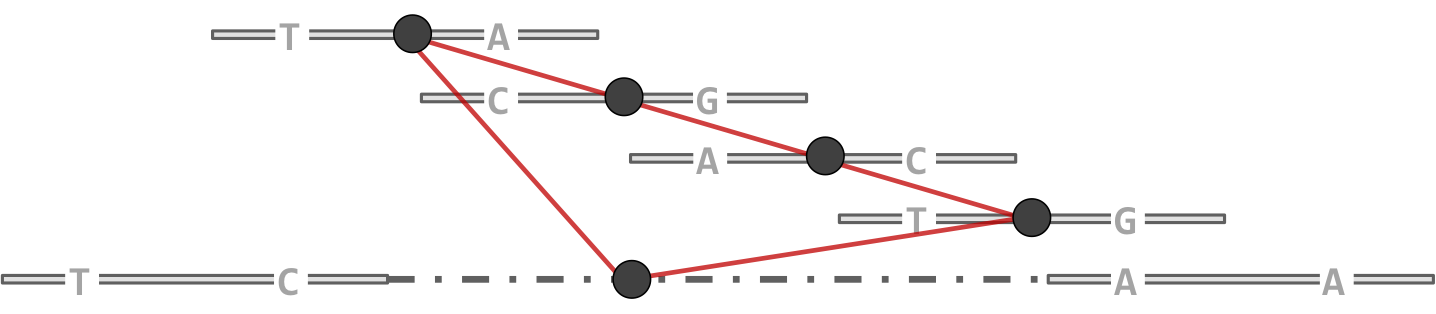
\includegraphics[width=0.6\textwidth]{graphics/mate-pair}\\
   NP-Hard\\
   \vspace{1em}
   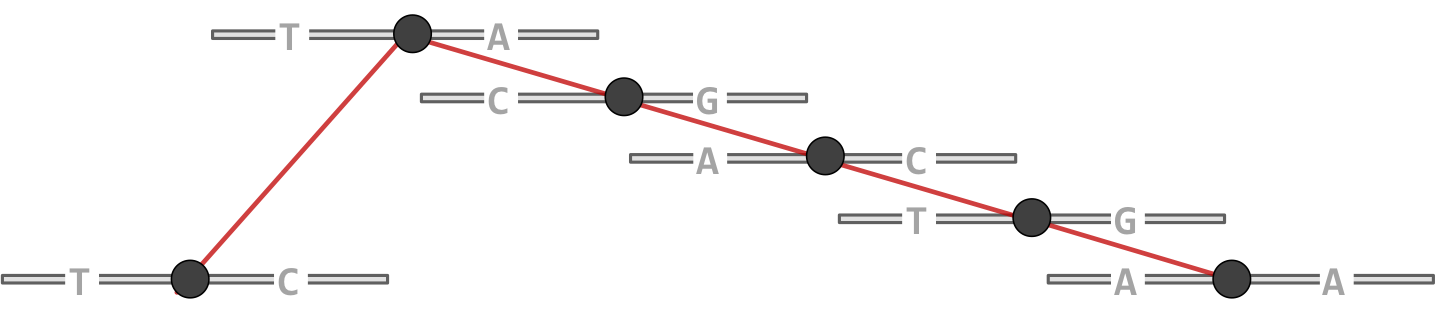
\includegraphics[width=0.6\textwidth]{graphics/mate-pair_broken}\\
   Polynomial Time
   \caption{The minimum coloring problem is polynomial time in this case if we ensure that reads are contiguous, without ``gaps.'' This, however, 
   means that mate-pair information cannot be fully used: we must associate mated reads with different graph nodes, such that they can possibly
   be associated with different haplotypes.}
   \label{matePairs}
\end{figure}


%% Figure of mate-pair NP-hard version

%% Figure of mate-pair easy version

Hapler executes a number of steps, which can be summarized as follows:
\begin{enumerate}
	
	\item SNP-call. We may wish to only consider some variations as relevant for haplotyping, to ignore sequencing errors, for example. Hapler can 
	take a list of positions to use as SNPs, or can find its own using a variety of methods (see Section \ref{inputAndOptions}).
	
	\item Identify reads that don't conflict with anything. These reads are common to all haplotypes, are are collected together into a ``universal''
	haplotype that may have several gaps (where variation occurs).
	
	\item Identify haplotype blocks. If reads are too short to span invariant regions, then there is no way to associate a haplotype segment from
	one variant region to another. (More formally, we only perform haplotyping on connected components of the conflict graph).

\begin{figure}[!h]
\centering
   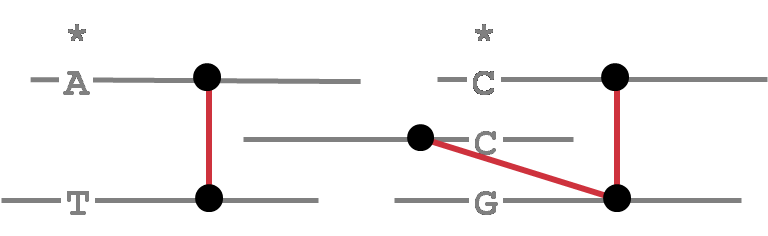
\includegraphics[width=0.4\textwidth]{graphics/haplotype_blocks}
   \caption{If there is more than one connected component in the conflict graph, no information exists to associate haplotypes from
   one connected component to another. Thus, Hapler only reconstructs haplotype regions for reads that are part of the same connected 
   component, which form contiguous ``haplotype blocks.'' Reads which occur between these and conflict with nothing are part of invariant
   regions; these are associated with a special ``universal'' haplotype for each multiple alignment (see Section \ref{output}).}
   \label{bicolor}
\end{figure}

	
	\item Minimally color the haplotype block conflict graphs. Hapler by default finds minimum colorings that also maximize the number of nodes 
	(reads) given colors all to themselves (reads that define a haplotype all by themselves). Since sequences containing errors could be viewed as 
	``haplotypes unto themselves,'' this is an effort to isolate sequencing error. (See Figure \ref{alternatecoloring}).	
	
	\item Repeated coloring. Because multiple such colorings (haplotypings) may be possible, Hapler repeats this process a number of 
	times, and only puts two reads into the same haplotype if they always are put together by the colorings. Increasing this parameter increases the
	confidence of haplotypes, avoiding chimeric reconstructions.
	
\begin{figure}[!h]
\centering
   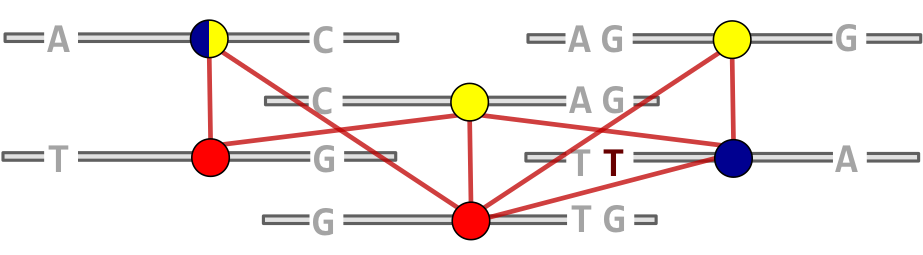
\includegraphics[width=0.4\textwidth]{graphics/two_haps_bicolor}
   \caption{There are many ways to minimally color a conflict graph; Hapler by default finds ways that also maximize the number of reads which 
   are left as colors (haplotypes) unto themselves. In this example, the upper left read may be given two possible colors: Hapler forces the use of
   yellow. This can be turned off by using \texttt{--maximize-one-read-haps false} (see Section \ref{inputAndOptions}). 
   Even so, in general multiple solutions may still be possible: Hapler pseudo-randomly samples from these and only infers haplotypes
   for reads which always appear similarly colored. The number of such samples is controlled with the \texttt{--random-repetitions} option.}
   \label{alternatecoloring}
\end{figure}

	
	\item Haplotype region assembly. For each haplotype an ``assembly'' is created, which is only defined for regions that are covered by reads assigned 
	to the
	haplotype. Undefined regions are left as `~'. For SNP-called loci, the majority allele within the haplotype (which will be invariant, i.e. a 
``unanimous'' vote) is used for the call. For Non-SNP-called loci, the majority
	vote of the alignment as a whole is used--this usually prevents sequencing error from getting into the haplotype reconstructions, since coverage 
	will be high overall but low for each individual haplotype.
	
	
	\item Minimum-chimerism consensus reconstruction. In most situations, the genetic diversity and coverage is not complete enough to create 
	haplotype regions which span the entire alignment with high confidence. However, we still want a ``consensus'' sequence that represents the 
	alignment, so we try to build such a sequence that minimizes the possibility of chimerism. One possible way of doing this is by looking at a 
	minimum tiling path over the haplotype regions, however, this is complicated by the existence of gaps in haplotype region assemblies as well 
	existence of the universal haplotype region (crossing into this isn't a real crossover and shouldn't be penalized). Thus, we aim to reconstruct 
	the full consensus only at SNP positions, filling in non-SNP loci with the majority vote of the overall alignment.\\
	
Given a consensus sequence $\mathcal{S}$, we define a ``possible crossover'' as any two adjacent SNP loci $i$ and $j$, where no haplotype
region supports (covers and agrees with) $\mathcal{S}$ at both $i$ and $j$.\\

Finding a consensus with minimal crossovers can easily be computed via dynamic programming: for each SNP locus $i$, we identify which
haplotype regions overlap it. We can then consider pairs of adjacent SNP loci in order, considering each possible configuration of haplotype usages
between them, and keeping track of the minimum chimeric path to that point---see Figure \ref{recon} for a representation. 

\begin{figure}[!t]
	\centering
		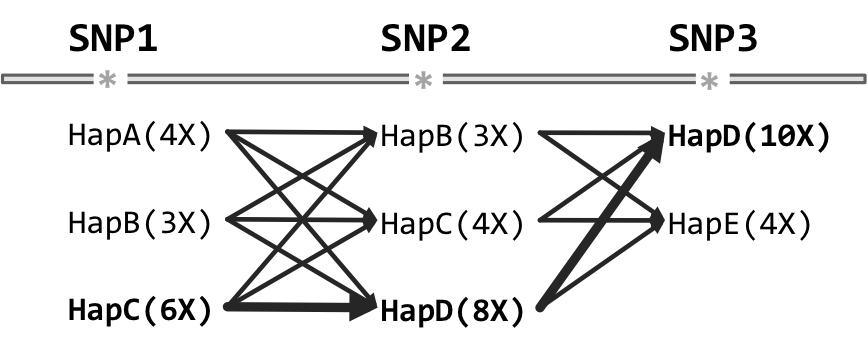
\includegraphics[width=0.4\textwidth]{reconstruction}
	\caption{Dynamic programming representation used for reconstructing minimum chimerism consensus sequences. At each SNP locus, the haplotype
	regions overlapping that locus are identified, and a minimum chimerism, maximum coverage path is identified. Shown are example haplotype
	regions overlapping for three SNPs, as well as the locus-specific coverages of each haplotype region. The bold path shows the optimal reconstruction;
	there is one crossover necessary which starts at the locus of SNP2 (HapC to HapD), the total maximized SNP coverage is $6+8+10=24$, and two unique
haplotype regions are used.}
	\label{recon}
\end{figure}


In fact, Hapler optimizes the consensus sequence $\mathcal{S}$ based on several criteria of decreasing importance:

\begin{enumerate}
	\item Minimizing the number of possible crossover points in $\mathcal{S}$.
	\item Maximizing the total supporting read coverage (both redundant and irredundant) of alleles used at SNP positions in $\mathcal{S}$.
	\item Minimizing the number of unique haplotype regions used.
\end{enumerate}

\item Evaluate the majority vote consensus and contigs given with \texttt{--evaluate-contigs} against haplotype regions. 
While Hapler can reconstruct a consensus minimizing 
possible chimerism, it can also evaluate any given consensus by computing the minimum amount of chimerism needed to reconstruct it from the haplotype
regions. The process is the same as above, except here for each SNP we only identify those haplotype regions overlapping \emph{and} agreeing with the
consensus before finding the optimal path. Also, in this case if the consensus has an allele at a SNP locus that isn't supported by any haplotype region,
a unique ``error haplotype'' is created specifically to cover that locus, incurring two crossovers (one into and one out of), unless that is the first or
last SNP.

\item Evaluate the Hapler consensus, majority vote, and given contigs against ground truth haplotypes. When the \texttt{--ground-truth}
option is used, Hapler also evaluates all consensus sequences against the ground-truth haplotypes to determining the ''true'' chimerism. 
This process is the same as above, except here ground-truth haplotypes are the bases for the path created rather than haplotype regions. 


\end{enumerate}



\appendix

\newpage
\section{Example TIGR Input Format}
\label{exampleTigrInputFormat}

The TIGR alignment format describes a multiple alignment of short reads against one or more longer consensus sequences. It is output by the Amos
tool \texttt{bank2contig} when working with an Amos Bank. 
For example, if the file \texttt{eidlist.txt} contains a number of contig identifiers
associated with an Amos Bank \texttt{bank}, one can simply run:

\begin{verbatim}
bank2contig -E eidlist.txt bank | java -jar Hapler.jar
\end{verbatim}

The TIGR format describes each multiple alignment starting with a \verb=##= line describing each consensus, followed by a number of \verb=#=
lines describing the placement of each read. Here is an example:

\begin{figure}[!h]
\centering
   \includegraphics[width=0.6\textwidth]{graphics/Example_tigr}
   \caption{Screenshot of example TIGR formatted input.}
   \label{exampleTIGR}
\end{figure}

Hapler currently only uses the following information from this format:  Contig IDs (for the multiple alignment names, \texttt{7180000000490} in the above),
Read Names (\texttt{FQVI7FG02F5V01} etc.), gapped read sequences, and read placement (numbers in \texttt{()}s: \texttt{239} and \texttt{452} in the above).

\newpage
\section{Example SAM Input Format}

\emph{NOTE: Hapler only takes as input SAM files against a gapped reference; it is currently not able to reconstruct an alignment if the CIGAR string indicates
that some reads have insertions relative to the reference (i.e., 'I' characters). In theory, one could parse \textbf{padded} SAM files, by replacing
insertion characters with match characters (which would ``match'' to a pad character in the reference). (From \url{http://www.projet-plume.org/files/SAM1.pdf}: ``
Note that it is hard to convert unpadded CIGAR to padded one. Fully resolving the alignment between inserted 
sequences would essentially require a  de novo assembler.'')}

\emph{Unfortunately, reference alignment tools which support mapping with indels such as BWA create unpadded SAM files against an ungapped/unpadded 
reference. We are currently working on the best way to resolve this issue; either by creating a converter or by finding some software to do the job (e.g.
Bambino claims to do this internally for viewing unpadded assemblies in SAM format). As a stopgap, one could use a reference aligner which doesn't support
mapping with indels, though we recognize this is a poor solution.}

\label{exampleSamInputFormat}

SAM is a relatively recent ASCII-formatted description of assembly/alignments. Each line represents a single read (which may be mated with another
read described in another line). Formal documentation can be found in \cite{LI2009}. The general form for each line is whitespace separated columns 
describing:

\begin{enumerate}
	\item Read Name
	\item Flag
	\item Scaffold Name
	\item Start Position (0 indexed, IIRC)
	\item Map Quality
	\item CIGAR alignment string (* if the read is not mapped and should be ignored)
	\item Mate Name
	\item Mate Position
	\item Insert Size
	\item Ungapped Sequence
	\item Quality Sequence
\end{enumerate}

SAM format specifies that mated reads will be given the \emph{same} name: this is how Hapler determines the existence of mate-pairs. 
If mate pairs are present, each read of a mate pair will be given a unique name by appending a number to the name:
\verb=_0=, \verb=_1=. (If there are multiple reads with the same name, this numbering scheme can continue).

\begin{figure}[!h]
\centering
   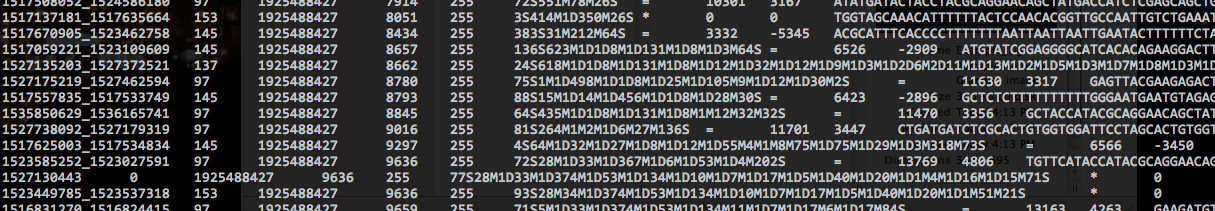
\includegraphics[width=\textwidth]{graphics/Example_sam}
   \caption{Screenshot of example SAM formatted input.}
   \label{exampleSAM}
\end{figure}

Hapler uses the Read Name and Start Position columns when parsing data. For the CIGAR string, the \verb=S= command necessitates a Soft Clip (sequence 
at the start or end that should be ignored), which is honored by Hapler. Hard clips (\verb=H=) are assumed to have already been done to reads, so 
Hapler ignores these. Values of \verb=N= are replaced with \verb=~= characters, which will cause cause sequences to be later split into separate 
sequences at those positions. Insert characters (\verb=I=) are not allowed: Hapler assumes that the multiple alignment is ``gapped.'' (If you are 
creating SAM files with \texttt{bank2contig} and run into this problem, try outputting in TIGR format instead). \verb=D= characters, which indicate 
deletion alleles w.r.t. the reference, cause Hapler to insert \verb=-= characters into the sequence. And of course, match characters (\verb=M=) are 
used to reconstruct the full gapped sequence from the ungapped sequence.

Hapler ignores Quality information in its current form.


\section{Example SNP Input Format}
\label{exampleSnpInputFormat}

Rather than using it's own internal SNP callers, Hapler can use user-provided SNP call loci. This is described in a simple text file with each row 
corresponding to a SNPs and the first column representing the name of the alignment the SNP is associated with and the second column being the 
0-indexed position of the SNP in the alignment. Note that any further columns in the file will be ignored. Duplicated SNPs and SNP calls which are 
non-variant in the actual alignment or are outside of the range of the alignment will produce warnings in the output, as will alignments for which no 
SNPs are called.

\begin{figure}[!h]
\centering
   \includegraphics[width=0.3\textwidth]{graphics/Example_snp}
   \caption{Screenshot of example SNP description format.}
   \label{exampleSAM}
\end{figure}


\bibliographystyle{plain}
\bibliography{khap}


\end{document}
